\documentclass[12pt,fleqn]{article}\usepackage{../../common}
\begin{document}
Ak�� Dinami�i

Euler ve Lagrange bak�� a��s� aras�ndaki farklarla ba�layal�m. Bu iki bak��
a��s� bir sivinin dinami�ini nas�l inceledi�imiz ile alakal�. E�er bir nehirdeki
kirlilik yo�unlu�unu �l��yorsak mesela, bunu herhangi bir $x,y,z$ noktas�nda
yapabiliriz, ve diyelim ki kirlilik belli bir yerde hi� de�i�miyor, ertesi g�n
gelsek ayn� yerde ayn� �l��m� al�yoruz [2, sf 78]. Bu yere bagimli Euler acisi.

Fakat farkli yerlerde farkli olcumler olabilir, mesela nehir boyunca bir kayik
icinde sabit hizda gidersek yogunluk lineer oranda artiyor. Bu durumda pir paket
siviyi takip ettigimizi dusunebiliriz, o paketin acisindan elde edilen olcumler
Lagrange bakis acisidir. 

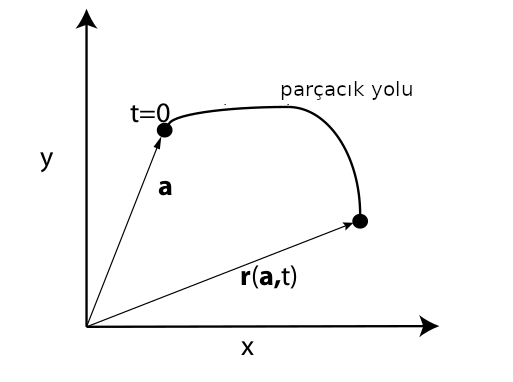
\includegraphics[width=20em]{phy_050_fluid_01.png}







[devam edecek]





Kaynaklar

[1] Bayramli, {\em Materyel T�rev, Euler ve Lagrange Bak�� A��s�},
    \url{https://youtu.be/XDrt-uATAY8}

[2] Storey, {\em Fluid Dynamics}

[3] Lumley, {\em Eulerian and Lagrangian Descriptions in Fluid Mechanics},
    \url{https://www.youtube.com/watch?v=mdN8OOkx2ko}

          
\end{document}
